% !TEX TS-program = pdflatex
% !TEX encoding = UTF-8 Unicode

\documentclass[]{beamer}
%\documentclass[aspectratio=169]{beamer}

\mode<presentation>
{
   \usetheme{edf}

  \setbeamercovered{transparent}

}
\beamertemplatenavigationsymbolsempty 

%gets rid of the footer and header, keep the frame numbering
\setbeamertemplate{footline}[page number]{}
\setbeamertemplate{navigation symbols}{}
\setbeamertemplate{headline}{}


\usepackage[french]{babel}


\usepackage[utf8]{inputenc}
\usepackage{hyperref}
%\usepackage{times}
\usepackage[T1]{fontenc}
\usepackage[absolute,overlay]{textpos}
\usepackage{subfigure}

\definecolor{gris}{rgb}{0.6,0.6,0.6}

%\usefonttheme{professionalfonts}
%\usefonttheme{serif}
%\usepackage{fontspec}
%\setmainfont{Avenir}

\TPGrid[0mm,0mm]{40}{30}
\title[Mesures cohérentes de susceptibilité...]{\\[1.7cm] Mesures cohérentes de susceptibilité d'un système en champ déterministe et en champ~aléatoire}

\author[E. Amador, C. Miry] 
{\\[-0.4cm]\footnotesize{E.~Amador, \and C.~Miry}\\[0.1cm]
\href{mailto:emmanuel.amador@edf.fr}{\scriptsize{\textcolor{gris}{\texttt{emmanuel.amador@edf.fr}}}}}


\institute[EDF lab] 
{\\[-0.4cm]
  \includegraphics[height=0.8cm]{img/EDFlab}\\[-0.2cm]
Centre R\&D des Renardières\\ Moret sur Loing}


\date[CEM 2014] 
{\\[0cm]\includegraphics[height=1.3cm]{img/LOGO_CEM_2014.png}}

\subject{EMC}

 \pgfdeclareimage[height=0.7cm]{edf-logo}{img/EDF}
 \logo{\pgfuseimage{edf-logo}}



\begin{document}

\begin{frame}
  \titlepage
\end{frame}

\begin{frame}{Sommaire}

  \tableofcontents

\end{frame}

\section{Contexte et motivations}
\begin{frame}{Contexte}
Nous souhaitons transférer les essais réalisés depuis plus de 20 ans en chambre anéchoïque (CA) vers des essais en chambre réverbérante (CRBM).
\begin{itemize}
    \item La fréquence maximale d'utilisation de la CA ne permet pas de couvrir tous les besoins,
    \item les mesures en CA sont longues,
    \item l'incertitude de mesure en CA est mal connue.
\end{itemize}
\end{frame}

\begin{frame}{Motivations}
La CRBM permet:
\begin{itemize} 
    \item des mesures entièrement automatisées,
    \item des mesures plus contraignantes (plus de chemins de couplages sont testés),
    \item une maîtrise de l'incertitude de mesure.
\end{itemize}
\end{frame}
\begin{frame}{Problématique}
Les mesures permettent la qualification d'un système pour son usage dans les sites de production d'EDF: 
\begin{itemize}
    \item les protocoles de mesure "maison" utilisant la CA doivent être adaptés à la CRBM,
    \item on doit assurer la continuité des résultats.
    \end{itemize}
 \begin{alertblock}{Problèmes}
 \begin{itemize}
 \item Les essais en CA et CRBM sont fondamentalement différents,
\item les marges d'erreur prévues dans les normes IEC 61000-4-21 et 61000-4-22, empêchent toute inter-comparaison pertinente des mesures.
\end{itemize}
 \end{alertblock}
\end{frame}
\begin{frame}{Solution}
\begin{itemize}
    \item En CRBM, le champ électrique rayonné est une quantité aléatoire dont les propriétés statistiques sont connues.
    \item En CA, le champ rayonné entre l'antenne d'émission et l'objet sous test (OST) est une quantité déterministe.
\end{itemize}
 \begin{exampleblock}{Solution ?}
Si le diagramme de susceptibilité d'un système est aléatoire, on peut considérer le couplage entre le champ incident déterministe et le système comme aléatoire.\\ Pouvons nous utiliser une approche commune pour la mesure en CRBM et en CA ?
 \end{exampleblock}
\end{frame}

\section{Éléments de théorie}
\subsection{Rayonnement d'un système quelconque}
\begin{frame}{Statistique du champ rayonné d'un système quelconque}
\begin{itemize}
    \item Nous cherchons à caractériser le champ lointain rayonné par un objet complexe,
    \item une sphère de rayon $a$ dotée de dipôles de Hertz quelconques placés aléatoirement à sa surface, simule un OST arbitraire~\cite{Wilson02},
    \item le nombre de dipôles $n$ et la taille électrique $ka=\frac{2\pi}{\lambda}a$ sont les paramètres de l'OST,
\item on génère un grand nombre d'OST afin d'extraire la statistique du champ rayonné par des objets sous test.

\end{itemize}
\centering
\begin{figure}
\includegraphics[trim=70 70 70 60,clip,scale=0.3]{./img/eut}
\caption{Un OST quelconque}
\end{figure}
\end{frame}

\begin{frame}{Rayonnement d'un objet  $a=1$ m et $n=100$ dipôles}
\begin{textblock}{14}(2,4)
\includegraphics[trim=110 180 90 90,clip,scale=0.24]{./img/rp_4.png}
\end{textblock}
\begin{textblock}{14}(22,4)
\includegraphics[trim=110 170 90 90,clip,scale=0.24]{./img/rp_24.png}
\end{textblock}
\begin{textblock}{14}(3,17)
\includegraphics[trim=110 180 90 90,clip,scale=0.24]{./img/rp_124.png}
\end{textblock}
\begin{textblock}{14}(22,17)
\includegraphics[trim=110 180 90 90,clip,scale=0.24]{./img/rp_249.png}
\end{textblock}
\end{frame}

\begin{frame}{Statistique du rayonnement d'objets quelconques}
\begin{textblock}{14}(3,4.5)
\centering
\includegraphics[trim=20 20 20 20,scale=0.35]{./img/CDF_ka_1_n_4.png}\\[0.2cm]
\tiny{$ka=1$, $n=4$}
\end{textblock}

\begin{textblock}{14}(22,4.5)
\centering
\includegraphics[trim=20 20 20 20,scale=0.35]{./img/CDF_ka_2_n_4.png}\\[0.2cm]
\tiny{$ka=2$, $n=4$}
\end{textblock}

\begin{textblock}{14}(3,16.5)
\centering

\includegraphics[trim=20 20 20 20,scale=0.35]{./img/CDF_ka_3_n_4.png}\\[0.2cm]
\tiny{$ka=3$, $n=4$}
\end{textblock}

\begin{textblock}{14}(22,16.5)
\centering
\includegraphics[trim=20 20 20 20,scale=0.35]{./img/CDF_ka_10_n_10.png}\\[0.2cm]
\tiny{$ka=10$, $n=10$}
\end{textblock}
\end{frame}

\begin{frame}{Les composantes de champ suivent-elles une distribution de Rayleigh?}
\vspace{-0.3cm}
\begin{figure}
\centering
\includegraphics[trim=0 0 0 0,clip,scale=0.45]{./img/TestAD}
\vspace{-0.3cm}
\caption{Probabilité d'observer une loi de Rayleigh, d'après le test d'Anderson-Darling sur $10^5$ tirages de Monte Carlo.}
\end{figure}
\end{frame}


\subsection{Mesure statistique de l'immunité d'un système}
\begin{frame}{Mesure statistique de l'immunité d'un système}
\vspace{-0.7cm}
\begin{figure}
\centering
\includegraphics[trim=20 0 10 20,clip,scale=0.35]{./img/rayleighCDF.png}
\vspace{-0.3cm}
\caption{Mesure statistique de la susceptibilité $E_s$ \cite{Amador13} d'un OST sous un champ dont les composantes suivent une loi de Rayleigh de moyenne $E_m$.}
\end{figure}
\begin{equation*}
E_s=2E_m\sqrt{\frac{\ln(1/p)}{\pi}}\text{\tiny{$\left[\approx 2E_m\sqrt{\frac{\ln(30/\color{red}{9}\color{black}{)}}{\pi}}\approx 1.2 E_m\right]$}}
\end{equation*}

\end{frame}
\section{Mode opératoire}
\subsection{Objet sous test}
\begin{frame}{Équipements sous test typiques}
\begin{itemize}
    \item Les mesures en immunité concernent souvent des équipements de grandes dimensions électriques placés dans des armoires électriques,
    \item l'absence de plan de masse sur les cartes électroniques et les mises à la terre vieillissantes des armoires rendent ces équipements particulièrement vulnérables aux ondes radio (téléphonie sans fil, WiFi...).
    \end{itemize}

\end{frame}
\begin{frame}{Mise au point d'un objet sous test générique}
\begin{figure}[t]
     \centering
     \subfigure[]{
          \label{fig_800}      
          \includegraphics[width=.47\columnwidth]{./img/EUT_ext.png}} 
    \subfigure[]{
          \label{fig_2000}
          \includegraphics[width=.47\columnwidth]{./img/EUT_int.png}}
     \caption{Vues extérieure (a) et intérieure (b) de l'objet sous test générique.}
     \label{fig_diags}
\end{figure}
\vspace{-0.2cm}
\centering{\textit{``Si le champ de la composante $z$ dépasse 10~V/m, on considère un défaut de l'OST.''}}
\end{frame}
\begin{frame}{Simulation du rayonnement de l'objet}
\subsection{Simulation du rayonnement de l'objet}
     \centering  
          \includegraphics[trim=0 10 0 18,clip,width=.3\columnwidth]{./img/EUT_ext.png}
\vspace{-0.8cm}
\begin{figure}[t]
     \centering
     \subfigure[]{
          \label{fig_800}      
          \includegraphics[trim=220 220 220 220,clip,width=.31\columnwidth]{./img/ka_800_44.png}} 
    \subfigure[]{
          \label{fig_2000}
          \includegraphics[trim=220 220 220 220,clip,width=.31\columnwidth]{./img/ka_2000_36.png}}
    \subfigure[]{
          \label{fig_4000}
          \includegraphics[trim=270 270 270 270,clip,width=.31\columnwidth]{./img/ka_4000_12.png}}
     \caption{Diagrammes de susceptibilité simulés dans CST de l'OST à 800~MHz (a), 2~GHz (b) et 4~GHz (c).}
     \label{fig_diagsCST}
\end{figure}
\end{frame}
\subsection{Mesures d'immunité}
\subsubsection{En chambre anéchoïque}
\begin{frame}{Mode opératoire en chambre anéchoïque}
\begin{itemize}
    \item Mesure réalisée entre 800~MHz et 4~GHz (la fréquence maximale théorique de la CA est de  2~GHz),
    \item pour garantir une homogénéité du champ maximale, l'étalonnage de la chambre se fait pour toutes les fréquences testées,
    \item on tire aléatoirement $n$ angles d'incidence et une polarisation (verticale ou horizontale), dans l'un des trois plans orthogonaux coupant l'OST,
    \item un champ de consigne $E_m$ est appliqué à l'OST (5, 10, 20, 40, 80~V/m).
\end{itemize}
\end{frame}
\subsubsection{En chambre réverbérante}
\begin{frame}{Mode opératoire en chambre réverbérante}
\begin{itemize}
    \item Mesure réalisée entre 800~MHz et 4~GHz,
    \item le facteur de qualité est mesuré pour chaque fréquence testée afin d'améliorer l'incertitude des mesures,
    \item on réalise la mesure en $n$ positions de brasseur,
 \item les valeurs moyennes d'une composante cartésienne du champ électrique $E_m$ sont appliquées successivement à l'OST (5, 10, 20, 40, 80~V/m).
\end{itemize}
\end{frame}
\section{Résultats}
\begin{frame}{Résultats pour $n=30$ observations}
     \centering 
\vspace{-0.1cm}
 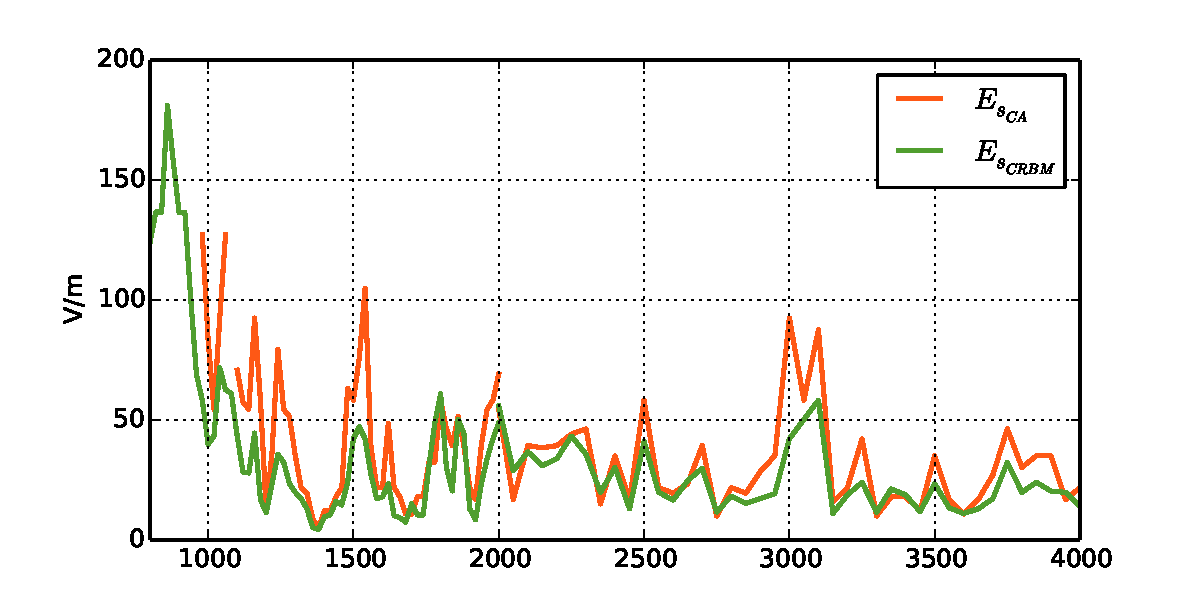
\includegraphics[trim=10 13 00 15,clip,width=.70\columnwidth]{./img/mesures_a30pres} \\[-0.2cm]
 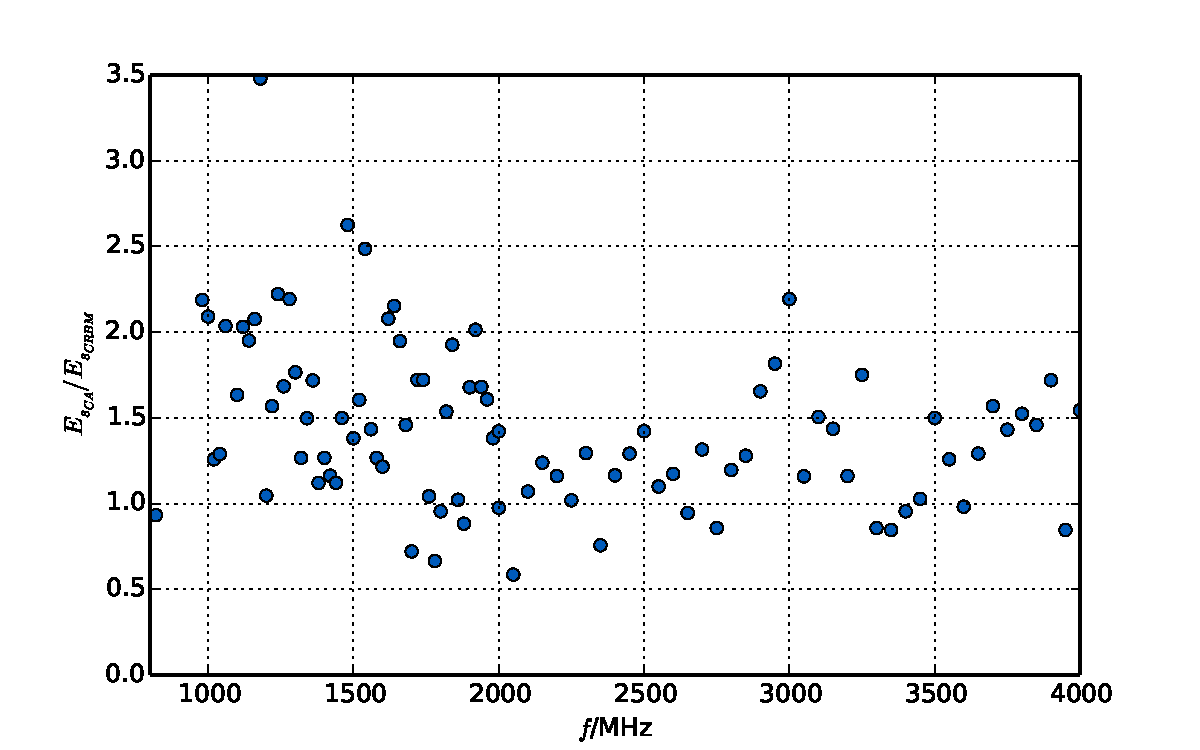
\includegraphics[trim=10 00 00 15,clip,width=.70\columnwidth]{./img/mesures_b30pres}
\end{frame}
\begin{frame}{Résultats pour $n=10$ observations}
 \centering 
\vspace{-0.1cm}
 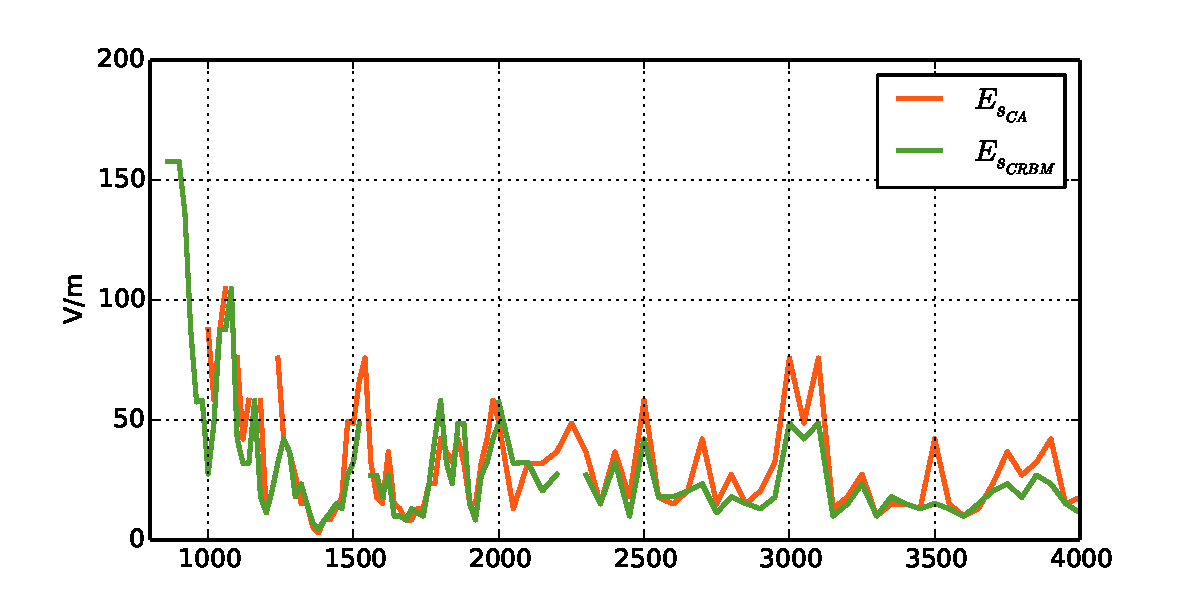
\includegraphics[trim=10 13 00 15,clip,width=.70\columnwidth]{./img/mesures_a10pres} \\[-0.2cm]
 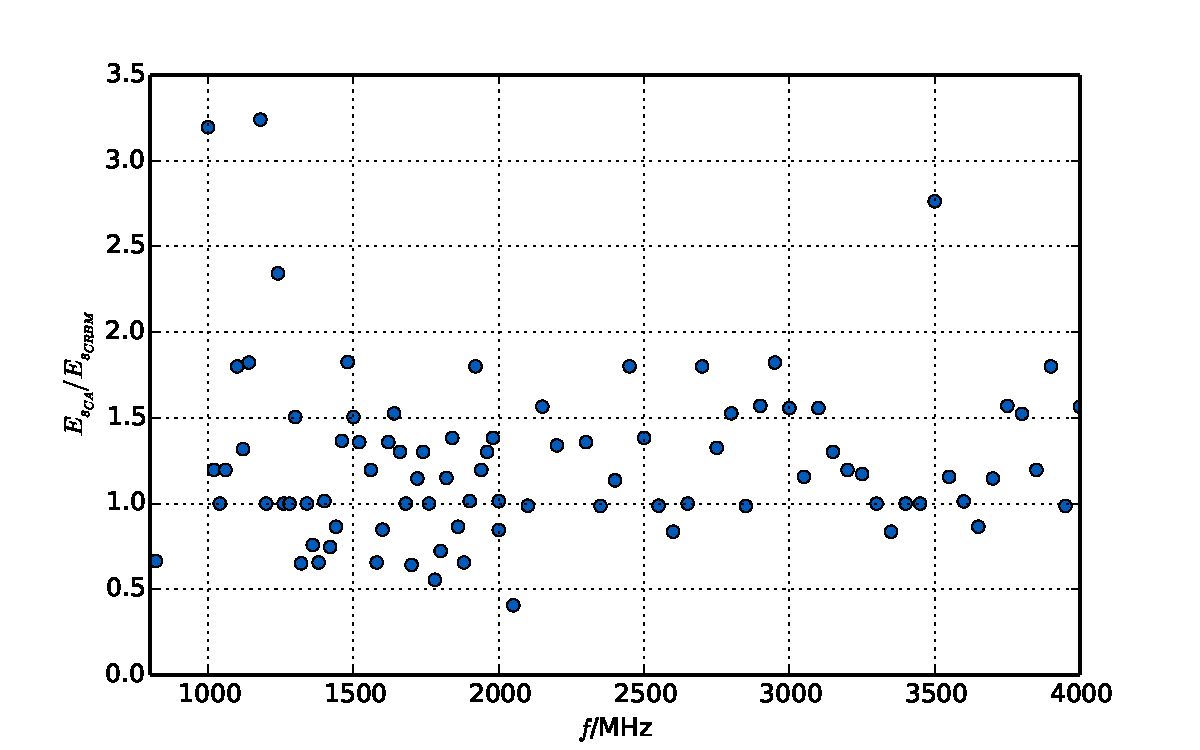
\includegraphics[trim=10 00 00 15,clip,width=.70\columnwidth]{./img/mesures_b10pres}
\end{frame}
\section{Conclusion}
\begin{frame}{Conclusion}
\begin{itemize}
    \item La méthode de mesure de susceptibilité développée pour la CRBM \cite{Amador13} peut s'appliquer à la CA et permet d'obtenir des mesures cohérentes :
	\begin{itemize}
	\item à condition  de disposer d'un OST suffisamment grand et ``complexe'',
	\item en réalisant un étalonnage des moyens d'essais plus précis que ce que préconisent les normes 61000-4-21/22.
	\end{itemize}
    \item avec cette approche plus robuste des mesures, nous pouvons réaliser des essais au delà de la fréquence maximale théorique de la CA,
    \item ces mesures peuvent être intégrées facilement à un essai normatif à condition de ne pas s'arrêter au premier défaut constaté pour estimer une probabilité de défaut.
\end{itemize}
\end{frame}
\begin{frame}{Perspectives}
\begin{itemize}
    \item Cette méthode de mesure est utilisée en CA et CRBM afin d'obtenir des mesures concordantes sur les mêmes OST,
    \item en donnant une dimension statistique aux mesures en CA, on peut réduire les incertitudes de mesure et ainsi mesurer des dérives légères de l'immunité d'un système, 
    \item on pense appliquer cette approche pour mesurer l'effet du vieillissement d'un composant sur ses propriétés électromagnétiques.
\end{itemize}
\end{frame}
\section{}
\begin{frame}{}
\setbeamertemplate{bibliography item}[text]
\bibliographystyle{ieeetr}
\small
\bibliography{IEEEabrv,biblio}
\vspace{0.3cm}

\begin{itemize}
\item Mesures réalisées avec Python et PyVisa, simulations de Monte~Carlo réalisées avec Python/Numpy et Julia:\\[0.2cm]
\centerline{\includegraphics[trim=150 120 120 60,clip,width=.2\columnwidth]{./img/python_logo.png}
\hspace{1cm}\includegraphics[width=.10\columnwidth]{./img/julia.png}}
\item Cette présentation, les données et les codes numériques sont disponibles à cette adresse:\\[0.2cm]
\centerline{\href{https://github.com/manuamador/CEM-2014}{{\texttt{https://github.com/manuamador/CEM-2014}}}}
\end{itemize}
\end{frame}

\begin{frame}{Incertitude de l'estimation}
\vspace{0cm}
\begin{figure}
\centering
\includegraphics[width=0.85\columnwidth]{./img/figErrbc.png}
\vspace{-0.3cm}
\caption{Intervalles de confiance à 95\% pour $n=10$, 30 et 150 observations.}
\end{figure}
\end{frame}


\end{document}



